\chapter*{5. Validación del motor}\addcontentsline{toc}{chapter}{5. Validación del motor}\label{cap:validation}

Para validar el correcto funcionamiento del prototipo y que cumple las expectativas deseadas en el diseño, se ha optado
por crear un minijuego en \glsentryfull{2d-es} y escenas de ejemplo en \glsentryfull{3d-es}.

\section*{5.1. Minijuego en \gls{2d-es}}\addcontentsline{toc}{section}{5.1. Minijuego en \gls{2d-es}}\label{sec:minigame}

El minijuego emula el famoso juego de móviles \textit{Flappy Bird}\cite{flappy-bird}, en el cual se controla un pájaro
que tiene que evitar obstáculos en forma de tuberías durante el máximo tiempo posible. Para variar la fórmula
se ha añadido un tiempo límite y monedas que el jugador tiene que recolectar para conseguir puntos. El nivel se
genera de forma procedural siendo en cada partida un nuevo desafío.

\subsection*{5.1.1. Estructura}\addcontentsline{toc}{section}{5.1.1. Estructura}\label{sec:minigame_structure}

\begin{figure}[h!]
    \centering
    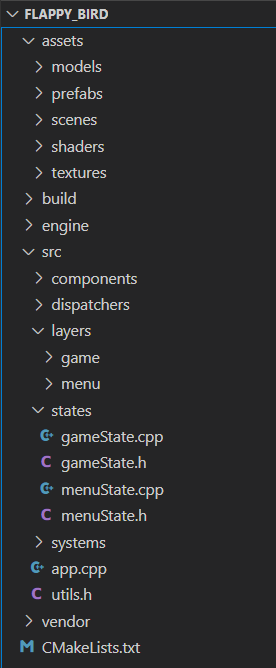
\includegraphics[scale=0.60]{minigame_structure}
    \caption{Estructura del minijuego}
    \label{minigame_structure}
\end{figure}
El proyecto presenta la siguiente estructura:

\begin{itemize}
    \item Assets: Recursos del proyecto: prototipos de las entidades, archivo escena, código \gls{glsl}, imágenes, etc.
    \item Build: Donde se crea el ejecutable.
    \item Engine: Código del motor de juegos.
    \item SRC: Código del minijuego.
    \begin{itemize}
    \item Components: Componentes de la escena.
    \item Dispatchers: Métodos para responder a los posibles eventos.
    \item Layers: Capas de cada estado del juego.
    \item States: Estados del juego.
    \item Systems: Sistemas de la escena.
    \item App.cpp: Conexión entre el código del usuario y el motor.
    \item Utils.h: Código auxiliar.
\end{itemize}
    \item Vendor: Librerías externas.
    \item CMakeLists.txt: Archivo para compilar el proyecto usando \textit{CMake}\cite{cmake}.
\end{itemize}

\subsection*{5.1.2. Estados}\addcontentsline{toc}{section}{5.1.2. Estados}\label{sec:minigame_states}

Cuando se ejecuta la aplicación se procede a la inicialización de todo el motor con la configuración,
inicializando el gestor de logs y cargando todos los \textit{assets}.

\subsubsection*{5.1.2.1. Menú}\addcontentsline{toc}{section}{5.1.2.1. Menú}\label{sec:minigame_menustate}
\begin{figure}[h!]
    \centering
    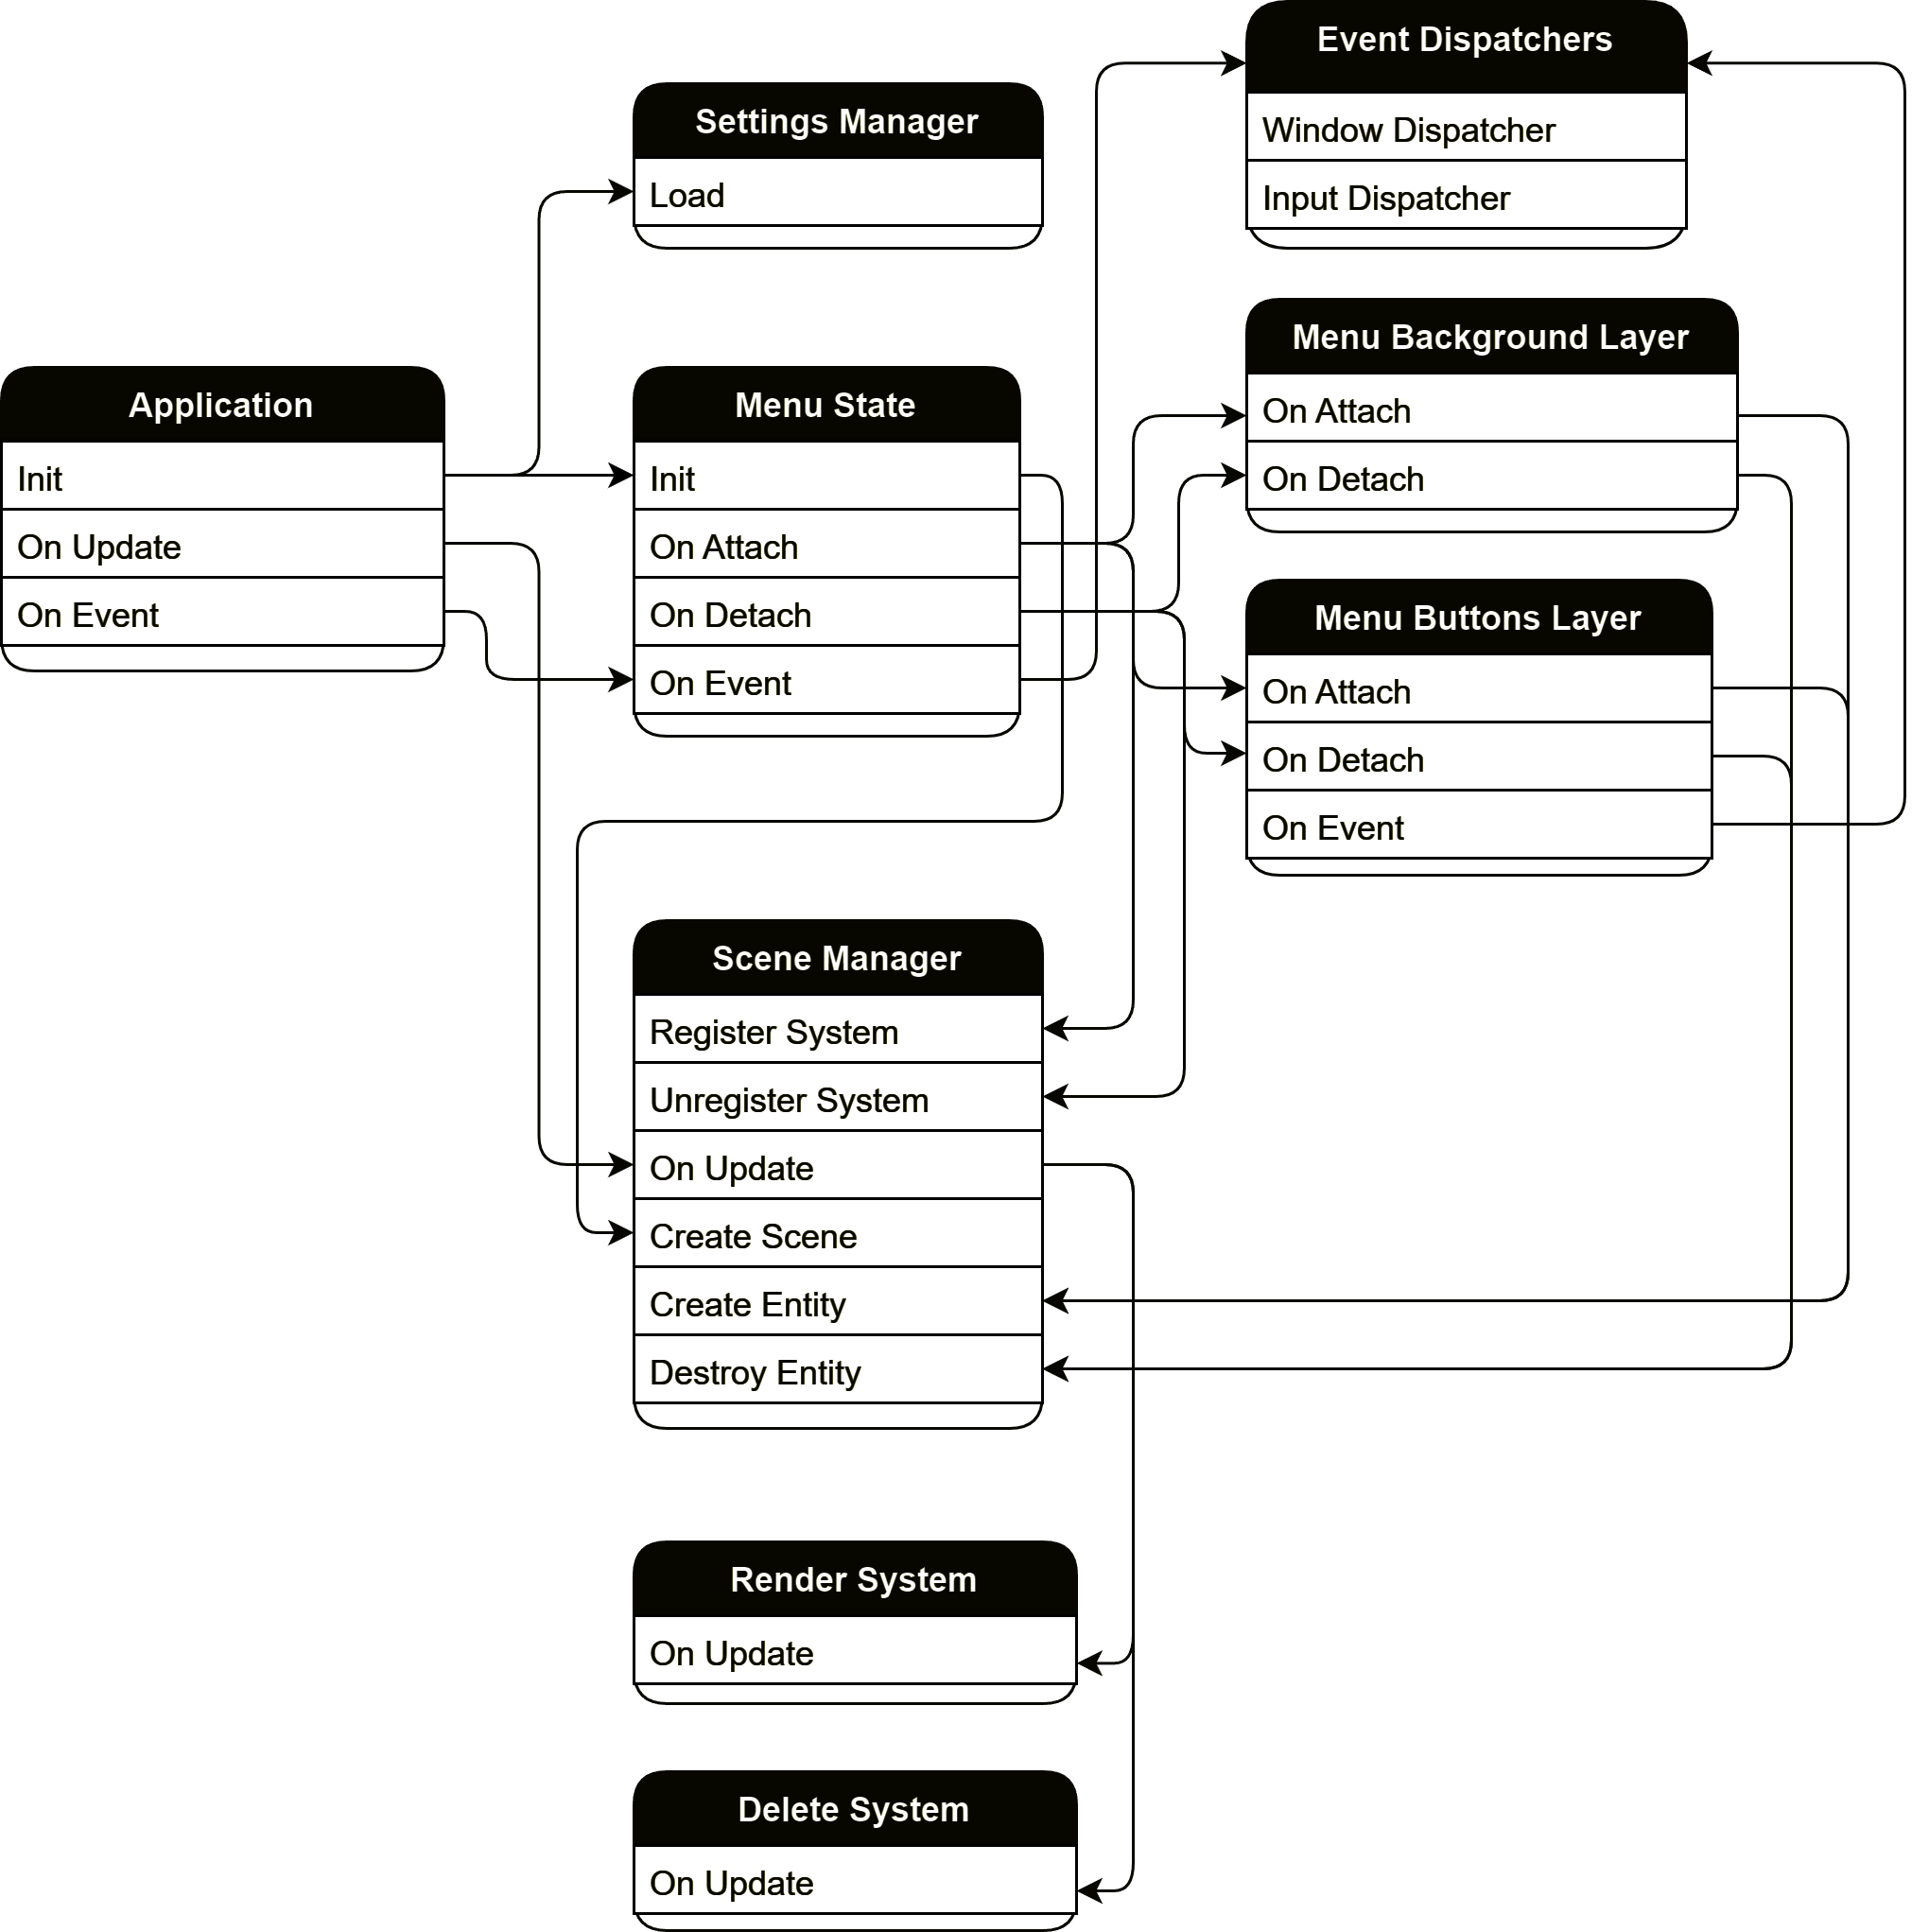
\includegraphics[scale=0.20]{minigame_menustate}
    \caption{Estado Menú}
    \label{minigame_menustate}
\end{figure}

Tomando como referencia la \figurename~\ref{minigame_menustate}, tras el inicio de la aplicación se carga
el estado inicial \textit{Menú}, creando la escena con sus entidades, componentes y sistemas. Las entidades serán
los aspectos visuales y botones como se puede ver en la \figurename~\ref{menu_visual}.

Habrá dos sistemas, el sistema \textit{render} con el dibujo o renderizado de la escena
y el sistema \textit{delete} que se encarga de limpiar el estado al salir del mismo.

Los eventos serán de ventana y teclado para interactuar con los botones del \textit{Menú}.

Por último, el estado se divide en dos \textit{layers}, el primero los aspectos visuales como el título y
el segundo los botones interactivo del \textit{Menú}.

\begin{figure}[h!]
    \centering
    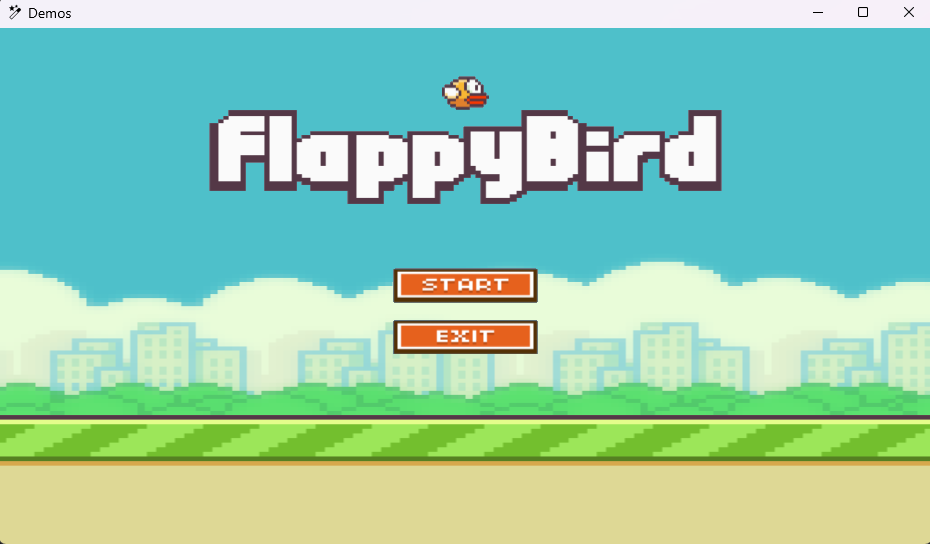
\includegraphics[scale=0.40]{menu_visual}
    \caption{Menú}
    \label{menu_visual}
\end{figure}

\subsubsection*{5.1.2.2. Juego}\addcontentsline{toc}{section}{5.1.2.2. Juego}\label{sec:minigame_gamestate}

Tomando como referencia la \figurename~\ref{minigame_gamestate}, desde el estado \textit{Menú} se pasa a su vez al estado \textit{Juego} al presionar el botón \textit{start}.
\begin{figure}[h!]
    \centering
    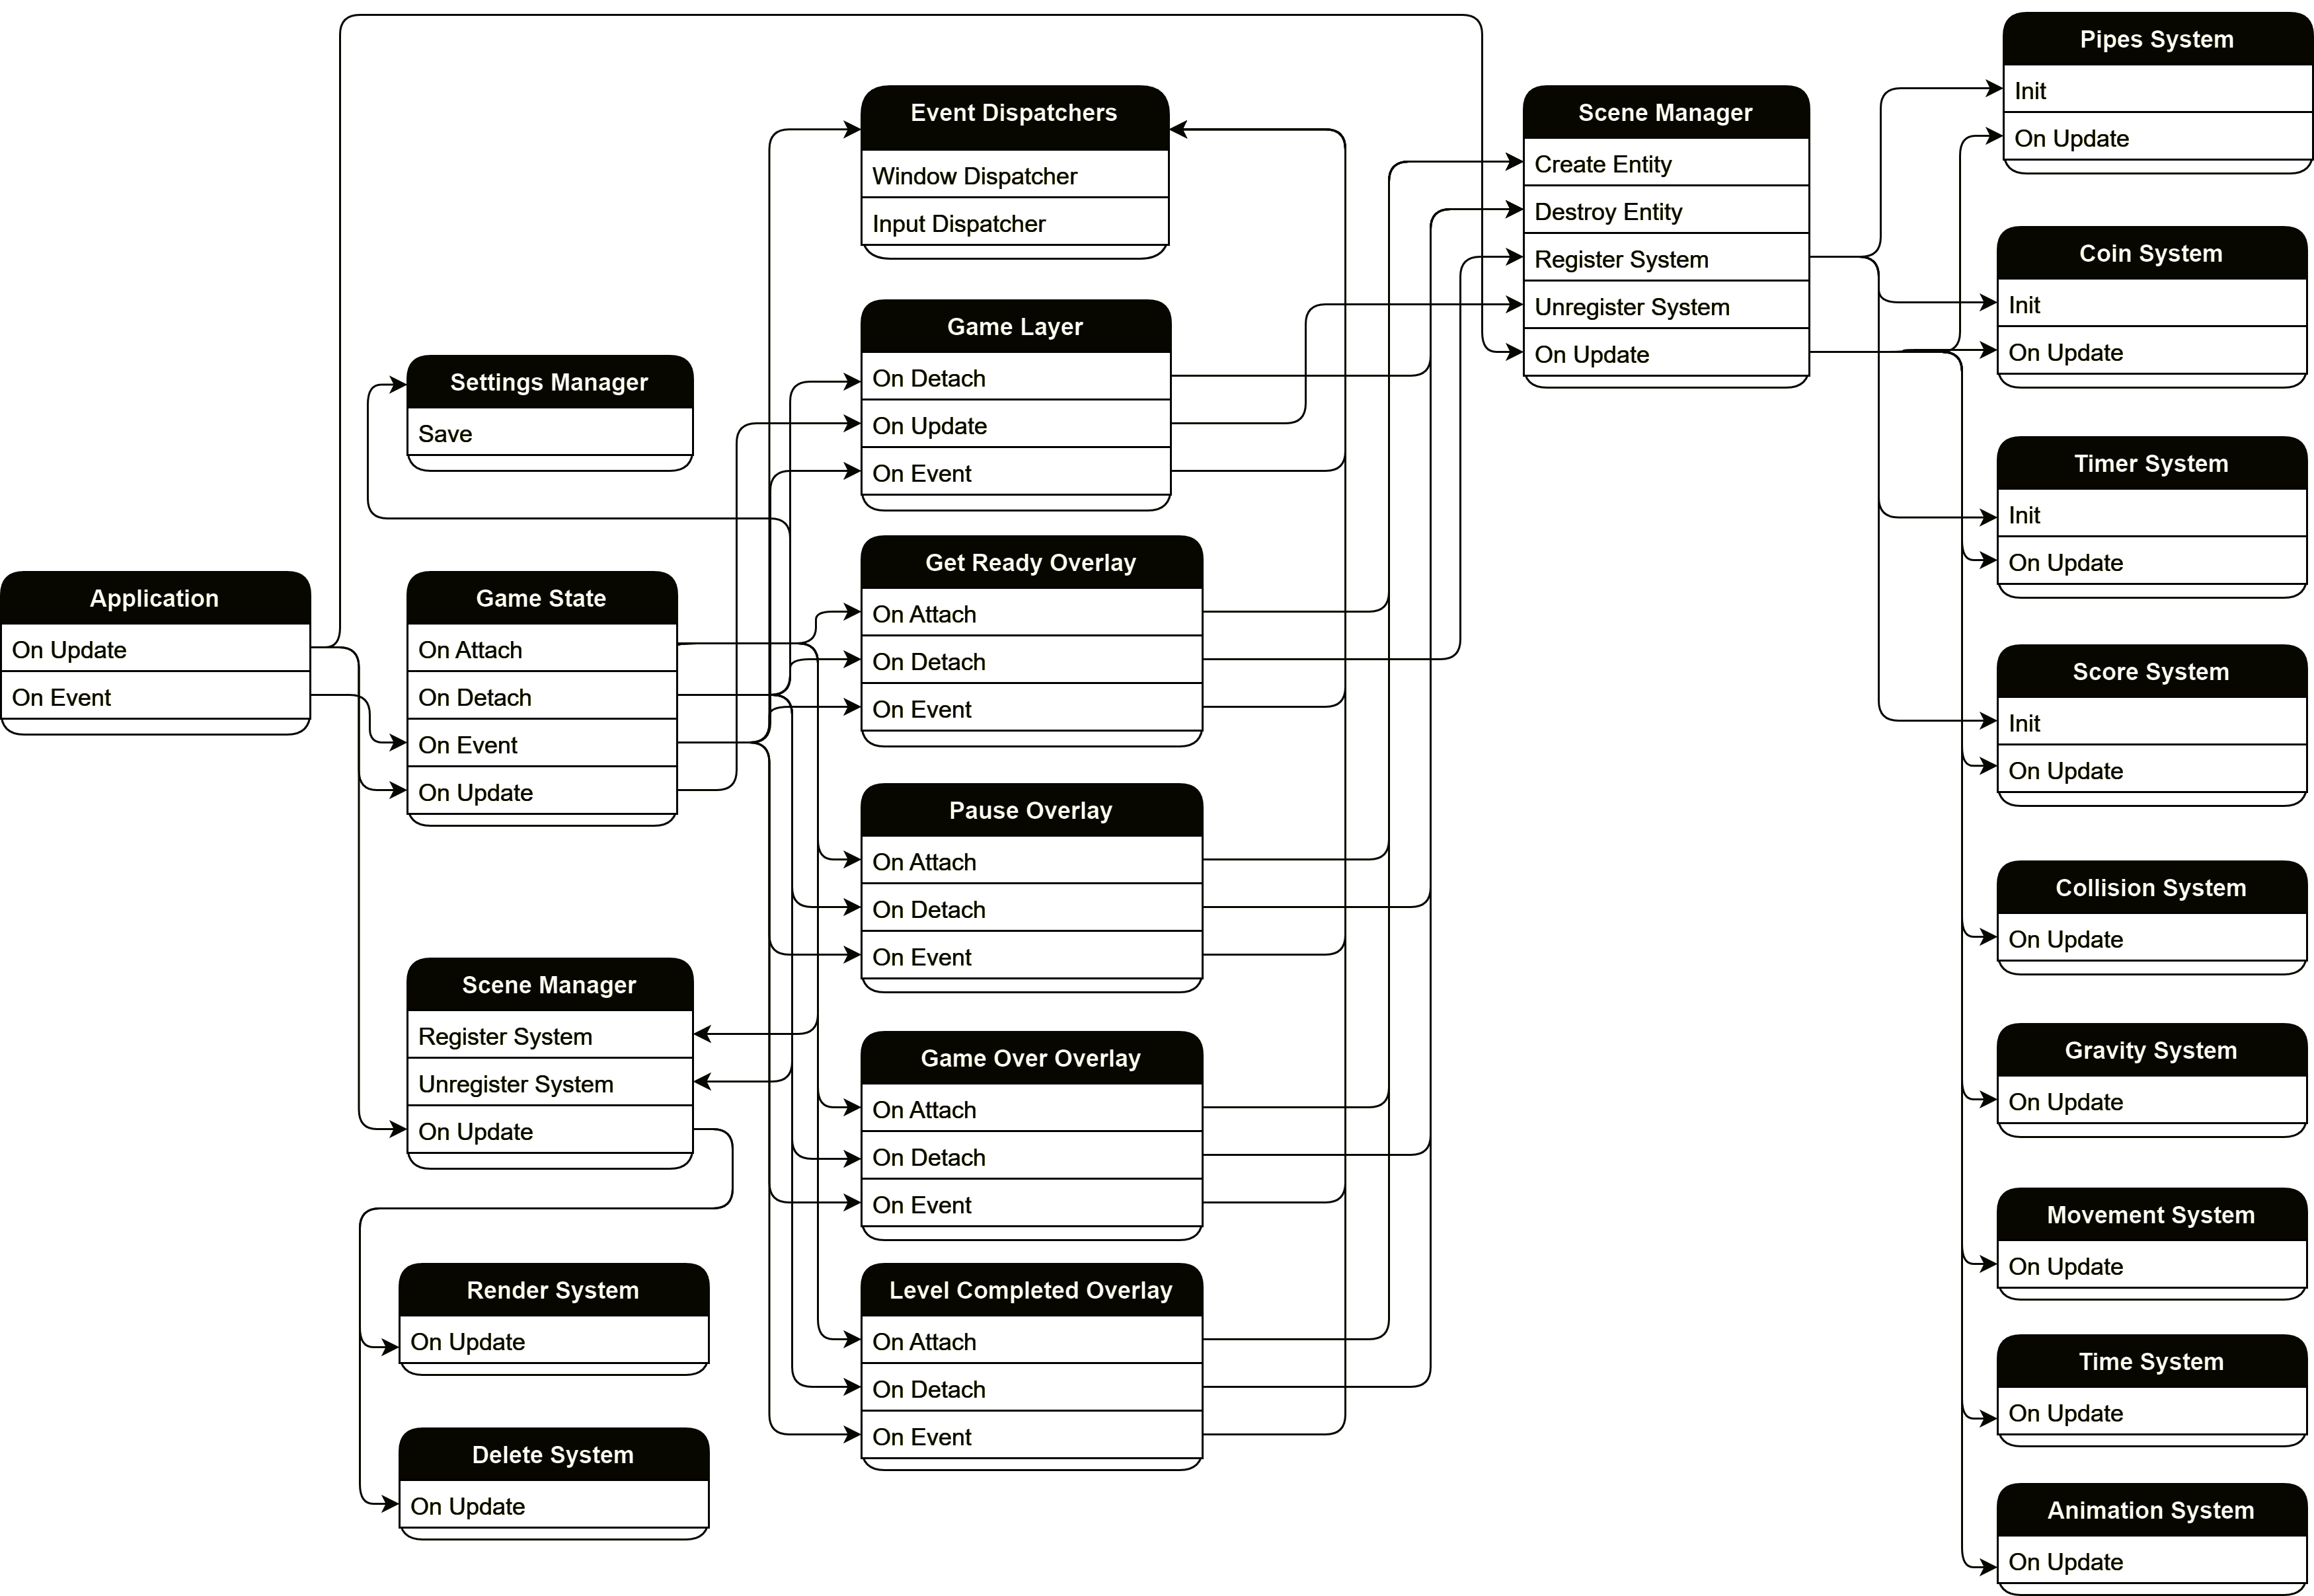
\includegraphics[width=1.11\linewidth]{minigame_gamestate}
    \caption{Estado Juego}
    \label{minigame_gamestate}
\end{figure}

El estado inicializará las entidades en la escena: tuberías, monedas, contador de tiempo, 
contador de puntuación, etc. Así como los sistemas: movimiento del jugador, gravedad,
colisión entre objetos, etc.
Por último el estado se compone de diferentes \textit{layers} y \textit{overlays}:
\begin{itemize}
    \item Carga del nivel \figurename~\ref{loading_visual}.
    \item Nivel del juego \figurename~\ref{gameplay_visual}.
    \item Pausa \figurename~\ref{pause_visual}.
    \item Game over \figurename~\ref{gameover_visual}.
    \item Nivel completado \figurename~\ref{completed_visual}.
\end{itemize}
\begin{figure}[h!]
    \centering
    \begin{minipage}[c]{.5\textwidth}
        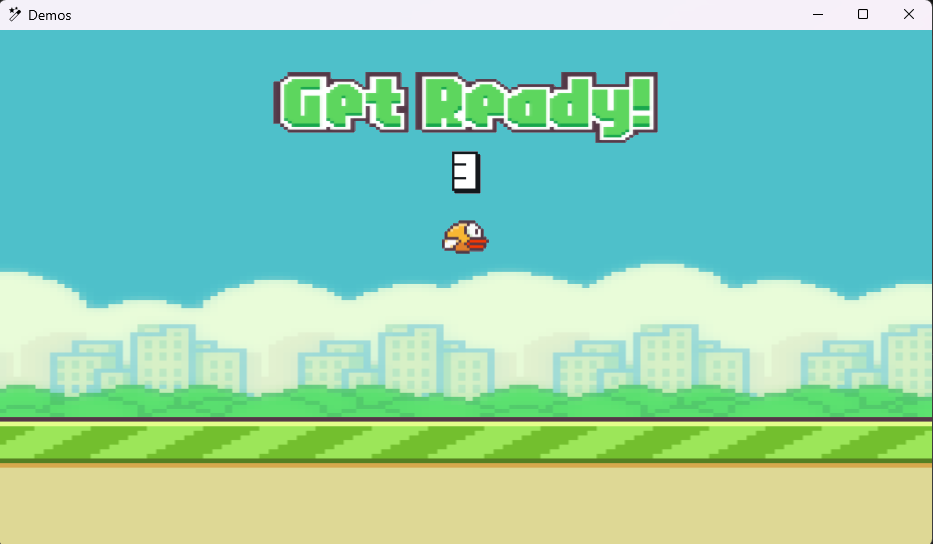
\includegraphics[scale=0.32]{loading_visual}
        \caption{Carga del nivel}
        \label{loading_visual}
    \end{minipage}%
    \begin{minipage}[c]{.5\textwidth}
        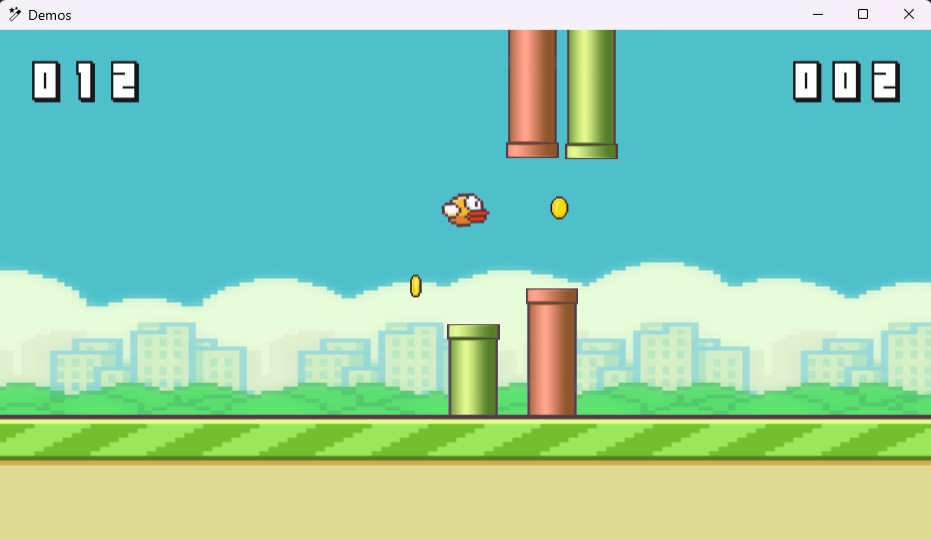
\includegraphics[scale=0.32]{gameplay_visual}
        \caption{Nivel del juego}
        \label{gameplay_visual}
    \end{minipage}%
\end{figure}
\begin{figure}[h!]
    \centering
    \begin{minipage}[c]{.5\textwidth}
        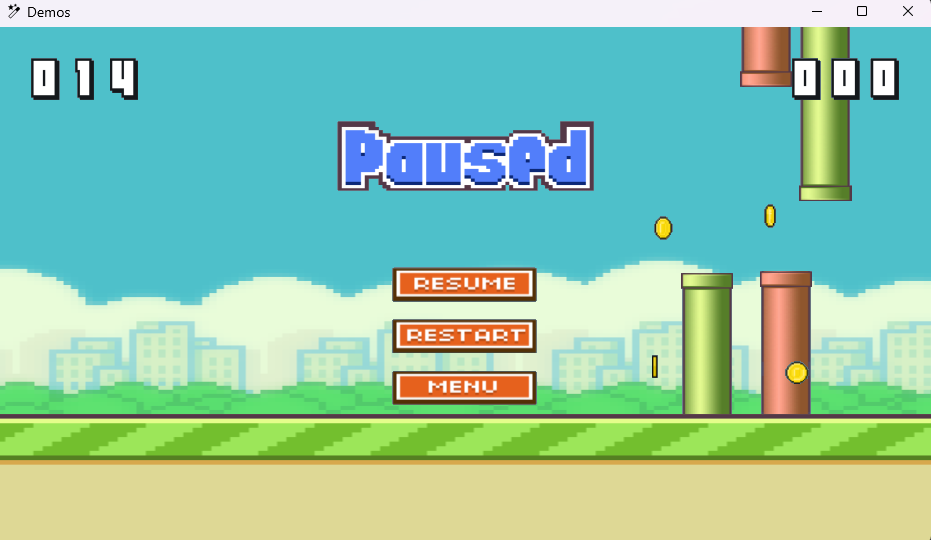
\includegraphics[scale=0.32]{pause_visual}
        \caption{Pausa}
        \label{pause_visual}
    \end{minipage}%
    \begin{minipage}[c]{.5\textwidth}
        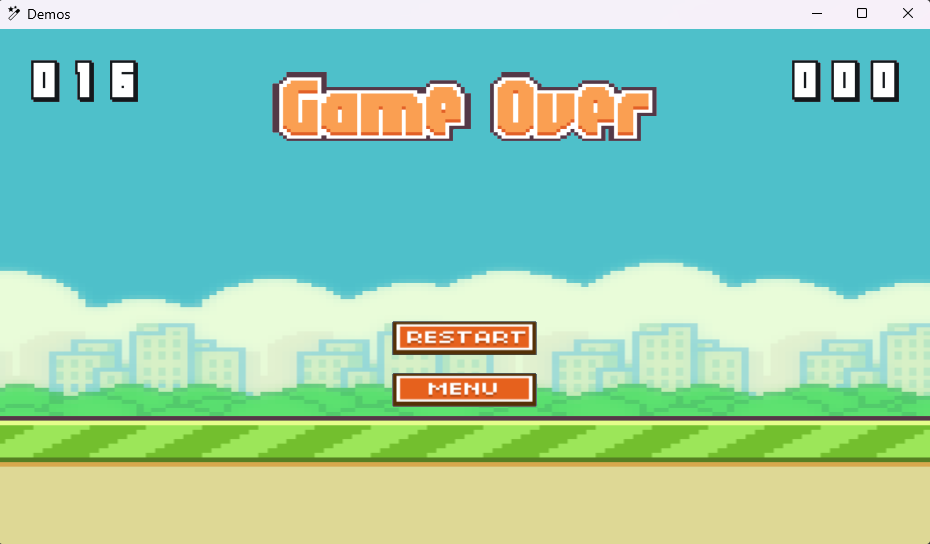
\includegraphics[scale=0.32]{gameover_visual}
        \caption{Game over}
        \label{gameover_visual}
    \end{minipage}%
\end{figure}
\begin{figure}[h!]
    \centering
    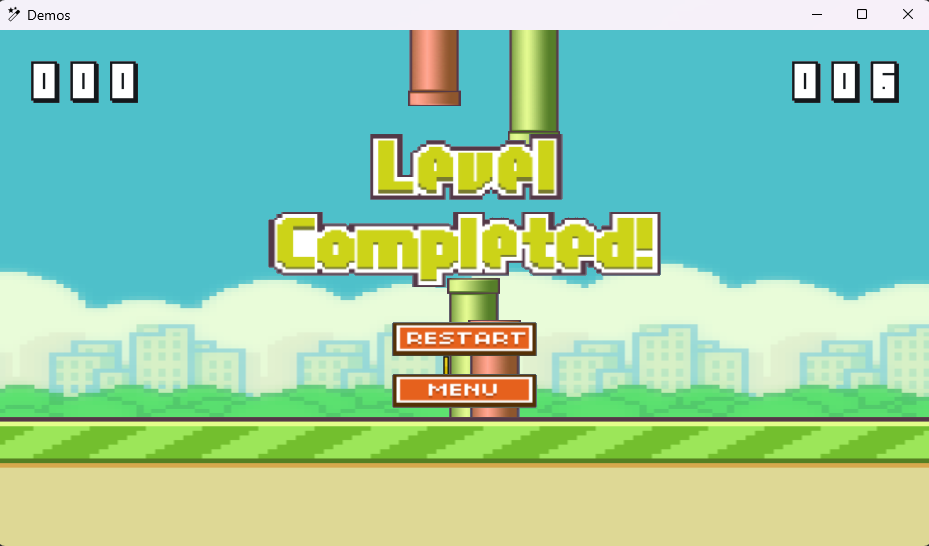
\includegraphics[scale=0.32]{completed_visual}
    \caption{Nivel completado}
    \label{completed_visual}
\end{figure}

\section*{5.2. Escenas en \gls{3d-es}}\addcontentsline{toc}{section}{5.2. Escenas en \gls{3d-es}}\label{sec:3d_scenes}

Para validar el motor en esta parte se presentan varias escenas de ejemplo probando carga de modelos, iluminación o
generación procedural entre otras para mostrar las capacidades del motor y lo que puede ofrecer al usuario.
Cada una de estas demostraciones se puede encontrar en la carpeta \textit{demos}.

\begin{figure}[h!]
    \centering
    \begin{minipage}[c]{.5\textwidth}
        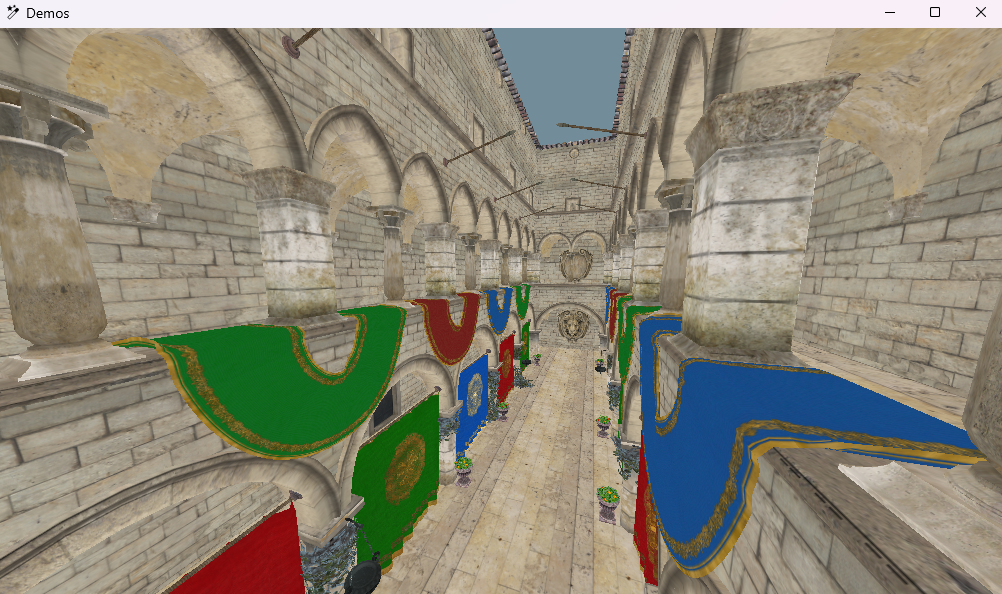
\includegraphics[scale=0.30]{sponza_visual}
        \caption{Escena palacio}
        \label{sponza_visual}
    \end{minipage}%
    \begin{minipage}[c]{.5\textwidth}
        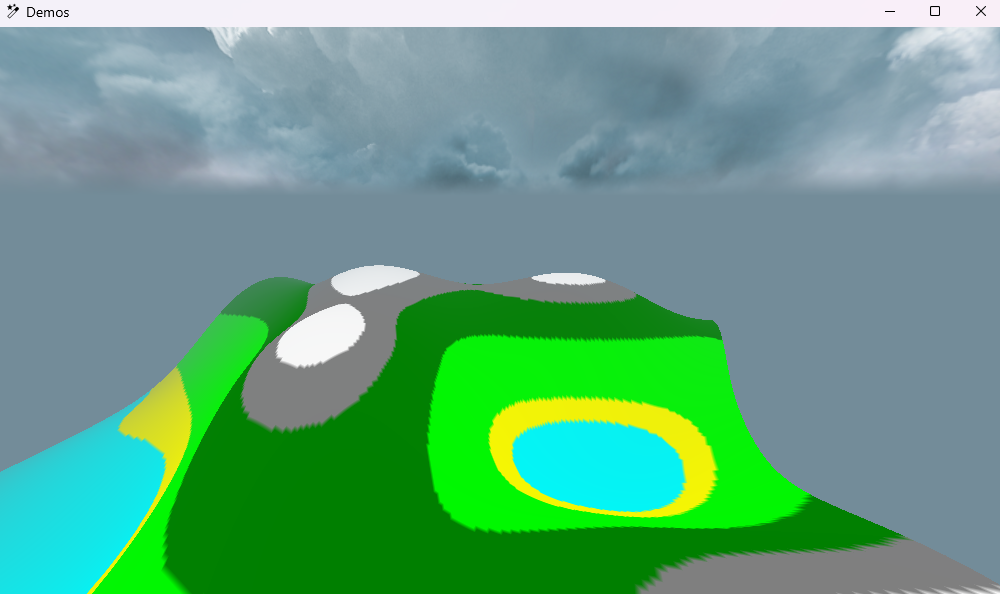
\includegraphics[scale=0.30]{procedural_visual}
        \caption{Escena generación procedural}
        \label{procedural_visual}
    \end{minipage}%
\end{figure}
\begin{figure}[h!]
    \centering
    \begin{minipage}[c]{.5\textwidth}
        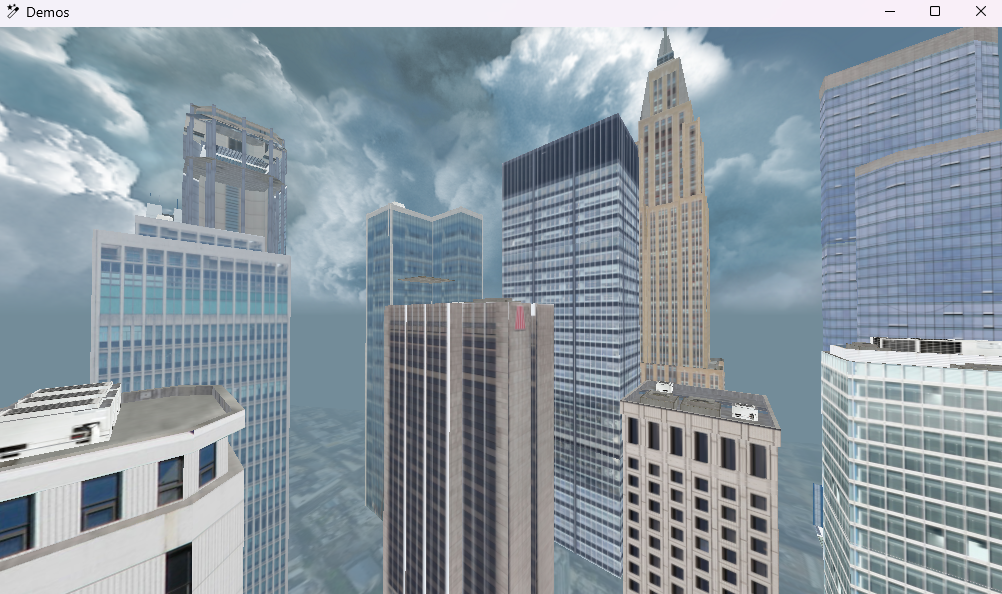
\includegraphics[scale=0.30]{skycrapers_visual}
        \caption{Escena rascacielos}
        \label{skycrapers_visual}
    \end{minipage}%
    \begin{minipage}[c]{.5\textwidth}
        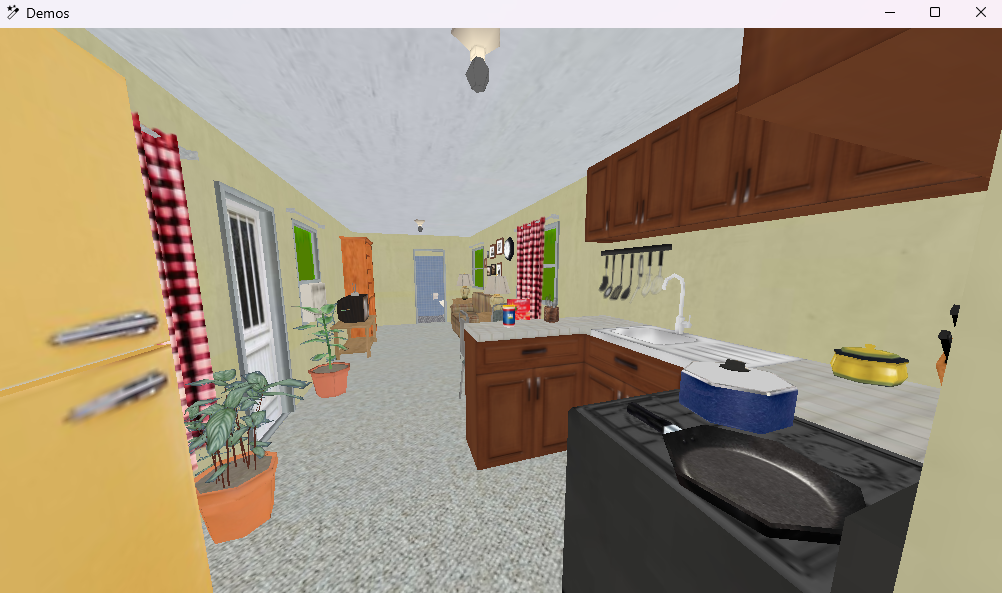
\includegraphics[scale=0.30]{room_visual}
        \caption{Escena habitación}
        \label{room_visual}
    \end{minipage}%
\end{figure}

\emptyPage